\label{chap:literature_survey}

\section{Introduction}
Post-disaster flood intelligence has experienced a profound technological evolution over the past decade. Driven by concurrent breakthroughs in unmanned aerial reconnaissance, deep semantic segmentation, foundation vision models, and large-scale language reasoning, research has transitioned from rudimentary manual photo-interpretation toward fully autonomous multi-modal intelligence systems. This chapter provides a rigorous, critical synthesis of the scholarly literature across four interrelated domains: (i) remote sensing and classical computer vision for flood water mapping, (ii) modern deep learning and foundation model segmentation architectures, (iii) Vision-Language Models (VLMs) for post-disaster scene understanding, and (iv) Retrieval-Augmented Generation (RAG) in disaster management and emergency decision support. The chapter culminates in an extensive comparative taxonomy table and articulates the fundamental research gaps addressed by the FloodSense framework.

\section{Remote Sensing and Classical Flood Mapping}
Early computational methodologies in flood extent mapping focused primarily on low-complexity spectral thresholding and morphological operations applied to satellite and aerial photography. Otsu's adaptive histogram thresholding algorithm~\cite{otsu1979threshold} has historically served as the benchmark baseline for binary water-land separation. By projecting RGB aerial images into color spaces such as HSV (Hue-Saturation-Value), LAB, or normalized difference water indices (NDWI in multispectral data), researchers identified that water bodies exhibit characteristic absorptions in the near-infrared spectrum and localized distributions in hue-saturation planes.

While classical thresholding requires minimal computational power and executes instantaneously on embedded microcontrollers, its efficacy collapses in complex, real-world post-flood environments:
\begin{enumerate}
    \item \textbf{High Inter-Class Spectral Variance:} Floodwaters in urban and rural environments are rarely pristine; they are laden with suspended silt, clay sediments, floating organic debris, and petroleum slicks, radically altering their spectral signatures.
    \item \textbf{Severe Shadow and Occlusion Confounds:} High-angle drone imagery of built environments features deep cast shadows from tall buildings and tree canopies. In hue and intensity spaces, building shadows frequently mimic muddy water bodies, generating massive false-positive inundation maps.
    \item \textbf{Inability to Discriminate Infrastructure Classes:} Color thresholding operates on independent pixel intensities without spatial contextual awareness. Consequently, it cannot differentiate a flooded road from a flooded building rooftop, severely undermining its utility for civil infrastructure damage assessment.
\end{enumerate}

\section{Deep Semantic Segmentation Paradigms}
The advent of deep Convolutional Neural Networks (CNNs) revolutionized remote sensing scene parsing. Pioneering architectures like U-Net and DeepLabv3+ utilized encoder-decoder topologies with atrous spatial pyramid pooling (ASPP) to capture multi-scale context. However, CNNs possess inherent inductive biases—notably localized receptive fields—that restrict their capacity to model long-range spatial dependencies across expansive aerial orthophotos.

\subsection{Vision Transformers and SegFormer}
To overcome the receptive field bottleneck of CNNs, Vision Transformers (ViTs) introduced self-attention mechanisms capable of modeling arbitrary pairwise pixel interactions across an entire image. Xie et al.~\cite{xie2021segformer} introduced \textbf{SegFormer}, a lightweight hierarchical Transformer architecture tailored specifically for semantic segmentation. SegFormer departs from traditional ViTs in several vital ways:
\begin{itemize}
    \item \textbf{Hierarchical Mix-Transformer (MiT) Encoder:} Instead of processing uniform non-overlapping patches, SegFormer generates multi-level feature representations at $\frac{1}{4}, \frac{1}{8}, \frac{1}{16},$ and $\frac{1}{32}$ of the original image resolution, capturing both fine structural details (such as lane markers and vehicle contours) and coarse environmental semantics.
    \item \textbf{Positional-Encoding-Free Design:} SegFormer employs $3 \times 3$ depthwise convolutions within feed-forward networks (Mix-FFN) to dynamically interpolate spatial locations, eliminating rigid positional embeddings and allowing the model to process arbitrary image dimensions without performance degradation during inference.
    \item \textbf{All-MLP Decoder:} Rather than relying on computationally heavy decoders, SegFormer aggregates multi-scale encoder features using pure Multi-Layer Perceptrons (MLPs), drastically reducing parameter counts while maintaining high representational capacity.
\end{itemize}

\subsection{Foundation Vision Models: SAM and SAM2}
A monumental paradigm shift occurred with the release of Meta's Segment Anything Model (SAM) by Kirillov et al.~\cite{kirillov2023segment}. Trained on the SA-1B dataset comprising over 1 billion masks across 11 million images, SAM demonstrated zero-shot generalization to unseen domains. The model utilizes a heavy Vision Transformer image encoder coupled with a promptable lightweight mask decoder that accepts points, bounding boxes, or text queries. 

Recently, Ravi et al.~\cite{ravi2024sam2} introduced \textbf{SAM 2}, extending the Segment Anything framework to continuous spatio-temporal video streams and high-resolution spatial tasks via streaming memory attention modules. Simultaneously, open-set object detection architectures such as \textbf{Grounding DINO}~\cite{liu2023grounding} merged contrastive language-image pre-training with DINO transformer decoders to perform arbitrary zero-shot text-prompted bounding box detection. When chained together (Grounding DINO $\rightarrow$ SAM / SAM2), this hybrid pipeline enables automated text-driven instance and semantic mask extraction without requiring fine-tuning on the target domain. However, as investigated in this thesis, zero-shot foundation models struggle with domain-specific aerial orthophotos, where tiny aerial vehicles and submerged roof geometries diverge drastically from natural ground-level photography.

\begin{figure}[htbp]
	\centering
	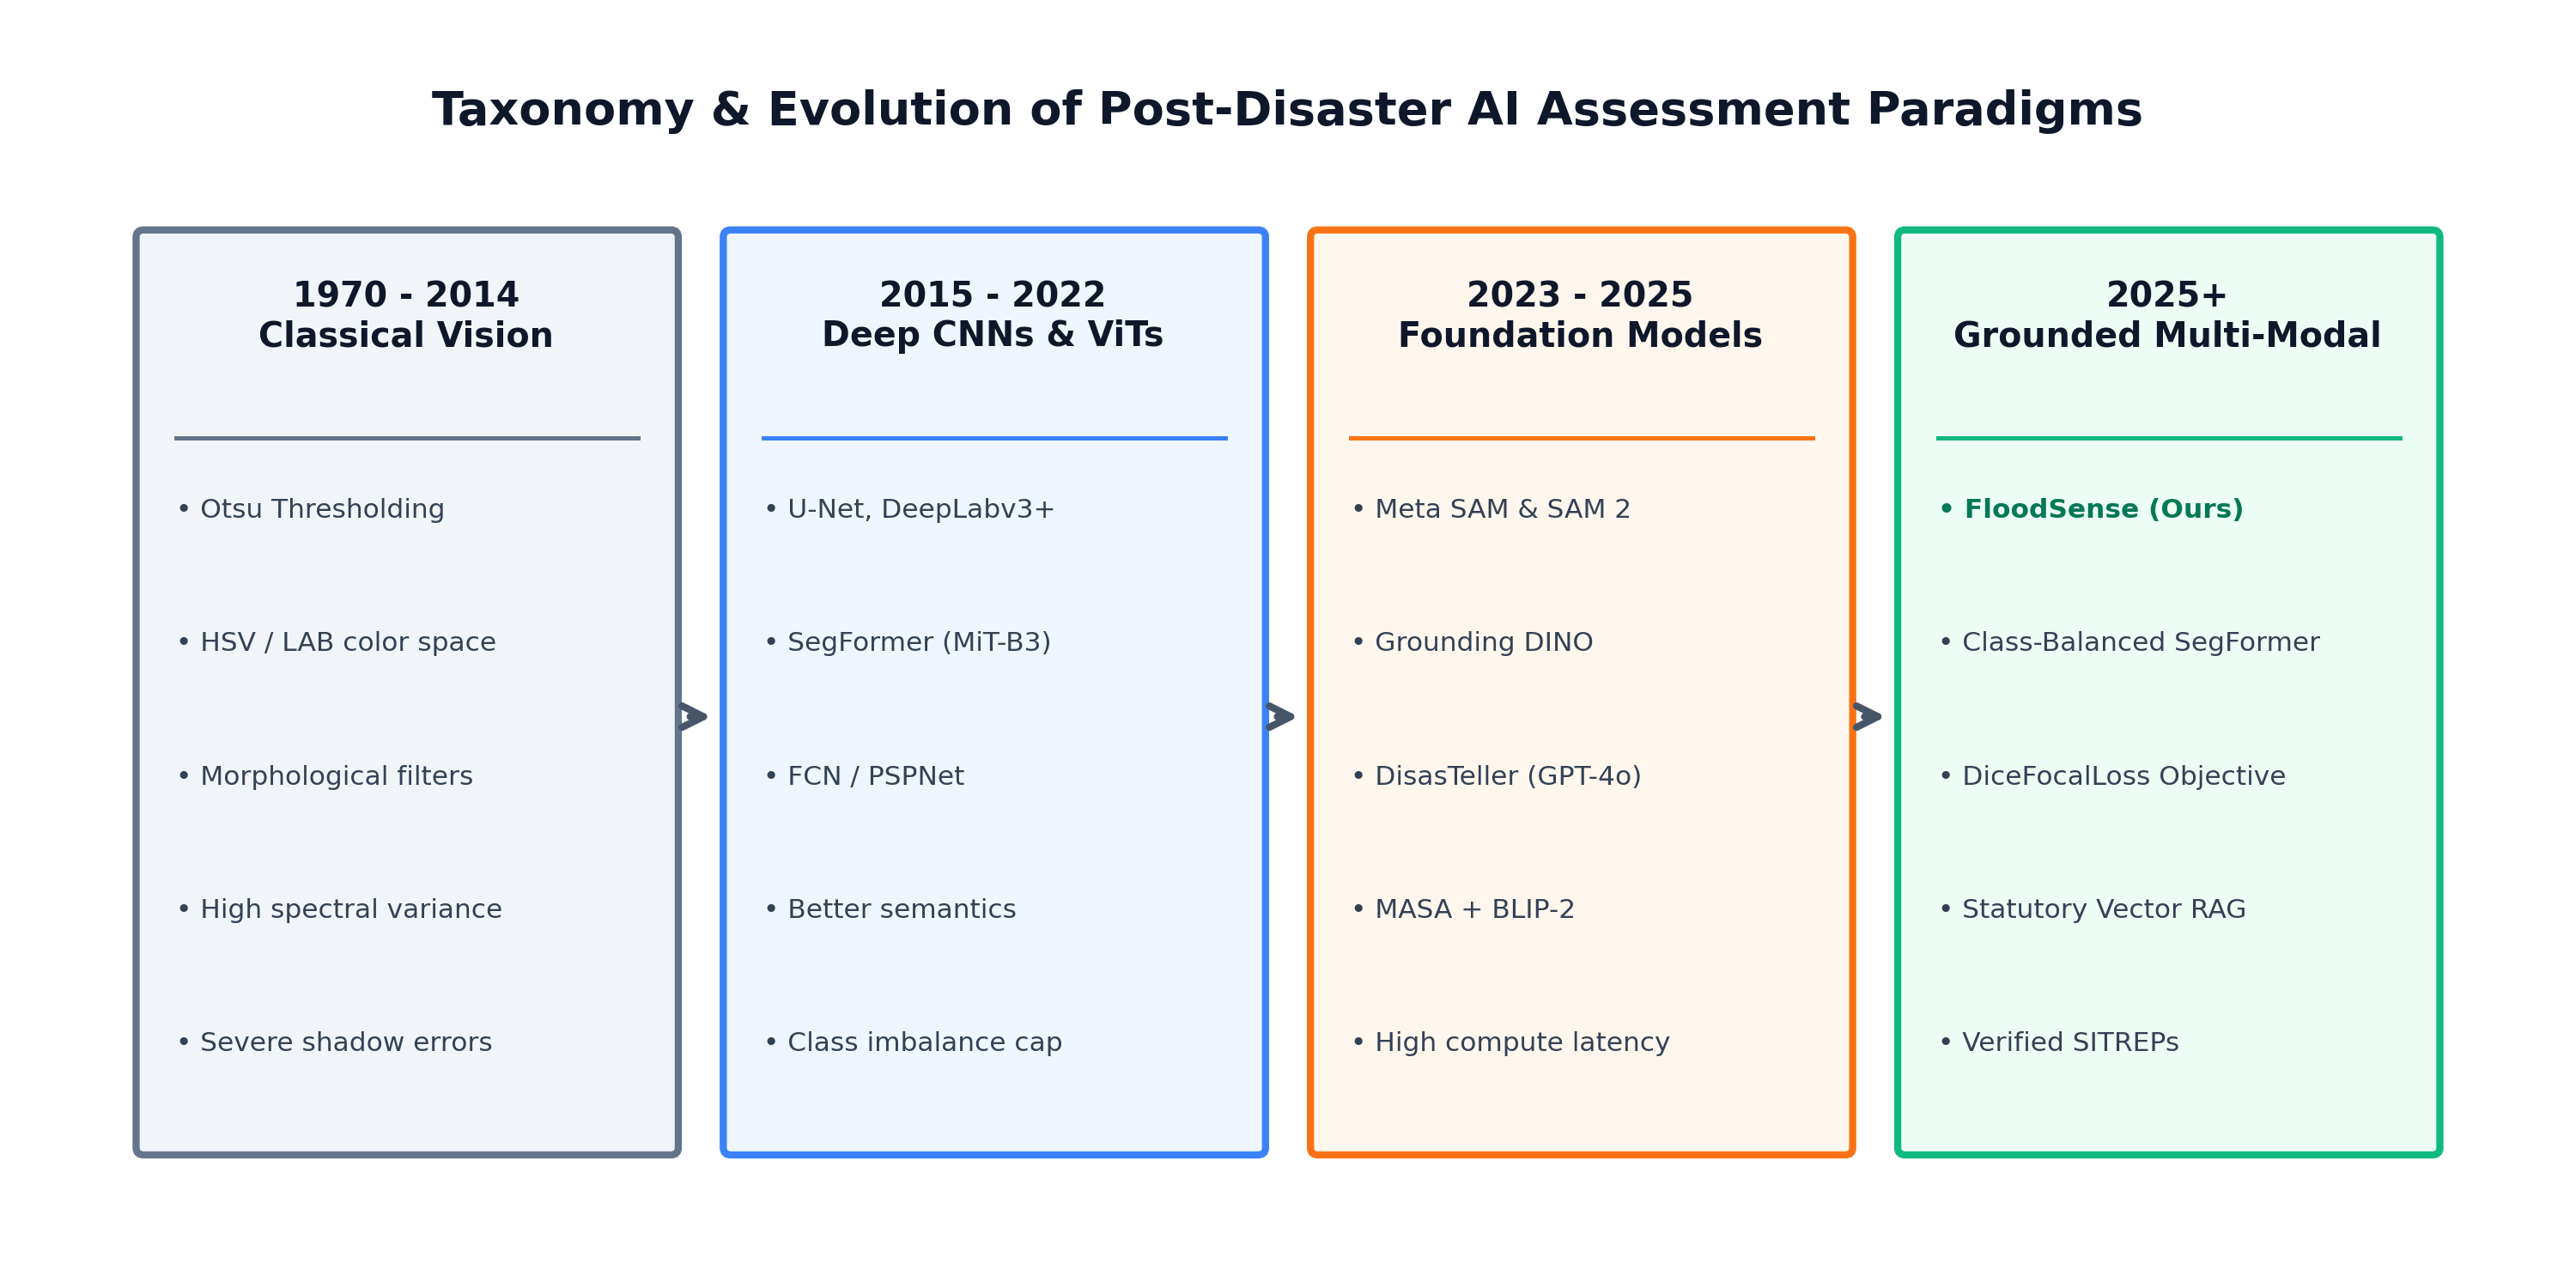
\includegraphics[width=0.92\textwidth]{images/fig2_lit_taxonomy.png}
	\caption{Evolution of Post-Disaster AI Paradigms: Historical progression from pixel-level thresholding to foundation vision models and multi-modal, protocol-grounded disaster intelligence.}
	\label{fig:lit_taxonomy}
\end{figure}

\section{Vision-Language Models (VLMs) in Disaster Assessment}
Recognizing the limitations of pure raster masks, researchers have explored Vision-Language Models to generate natural language explanations directly from disaster imagery.
\begin{itemize}
    \item \textbf{DisasTeller (2026):} Chen et al.~\cite{disasteller2026} proposed DisasTeller, a multi-agent framework employing Large Vision-Language Models (LVLMs) for post-disaster assessment and alarm creation. Evaluated on the Wajima City earthquake case study in Japan, the system coordinated four specialized agents with an internal RAG module. The authors demonstrated that frontier proprietary models like GPT-4o achieved a disaster grading score of $7.3/10$, outperforming open-weight models like Gemma-3 ($4.6/10$). However, the framework suffered from cascaded error propagation: errors in early-stage LVLM visual parsing corrupted downstream resource planning and alarm generation.
    \item \textbf{MASA + BLIP-2 (2026):} Aydin et al.~\cite{masa_blip2026} developed an explainable flood damage assessment pipeline integrating a Multi-Atrous Self-Attention (MASA) mechanism with a LoRA-fine-tuned BLIP-2 vision-language model. The system generated detailed textual captions regarding structural failure modes alongside segmentation masks, attaining an $80.77\%$ BLEU score. However, the linguistic output was restricted to generic image descriptions without integration into statutory emergency operations protocols.
    \item \textbf{LLMArk (2026):} Wu et al.~\cite{llmark2025} introduced LLMArk, an instance-aware 7-billion-parameter multimodal foundation model trained specifically for hydrological risk and built environment damage estimation on the VLFRA dataset. The model achieved superior zero-shot damage grading relative to general-purpose VLMs across 12 evaluation metrics, but lacked deterministic numerical estimation of damaged assets and spatial accessibility metrics.
    \item \textbf{DisasterM3 (2026):} Wang et al.~\cite{disasterm3_2025} curated a comprehensive benchmark consisting of 26,988 bi-temporal satellite and drone images spanning 9 disaster tasks. Their benchmark established that multi-task foundation models yield a $40.8\%$ improvement in referring expression segmentation, but confirmed that extreme class imbalance in flood scenes remains a severe unresolved obstacle.
\end{itemize}

\section{Retrieval-Augmented Generation (RAG) in Emergency Response}
While Large Language Models possess broad encyclopedic knowledge, their application in high-consequence disaster management is impeded by two fatal vulnerabilities: \textit{temporal staleness} and \textit{hallucination}. LLMs frequently fabricate plausible-sounding guidelines or cite non-existent emergency clauses. Retrieval-Augmented Generation (RAG), pioneered by Lewis et al.~\cite{lewis2020retrieval}, resolves these issues by grounding language generation in verified, externally retrieved document chunks.

In the emergency response literature, several pioneering RAG frameworks have emerged:
\begin{itemize}
    \item \textbf{CrisiSense-RAG (2026):} Xiao et al.~\cite{crisisense2025} proposed a multi-modal RAG system evaluated during Hurricane Harvey in Texas. By combining satellite SAR flood extent maps with municipal emergency response manuals, CrisiSense-RAG reduced flood extent estimation error by $8.62$ percentage points compared to unaugmented models.
    \item \textbf{Training-Free RAG (2026):} Huang et al.~\cite{trainingfree_rag2025} introduced a lightweight, training-free RAG approach using reinforced reasoning over indexed disaster case databases. Their architecture achieved an overall response accuracy of $0.668$ while proving $35.9\times$ to $81.9\times$ more cost-effective than fine-tuning proprietary frontier models.
    \item \textbf{RS-RAG (2026):} Wen et al.~\cite{rs_rag2025} designed a cross-modal satellite retrieval-augmented visual question answering system that attained $79\%$ classification accuracy on disaster queries by leveraging dense vector embeddings generated by Sentence-BERT~\cite{reimers2019sentence}.
\end{itemize}

\section{Literature Comparison and Taxonomy Table}
To contextualize the scientific positioning of FloodSense against the broader literature, Table~\ref{tab:lit_comparison} synthesizes key contemporary methodologies, detailing their core mechanisms, dataset benchmarks, reported metrics, and fundamental operational drawbacks.

\begin{table}[p]
\centering
\caption{Comprehensive Synthesis and Taxonomy of State-of-the-Art Post-Disaster AI Frameworks.}
\label{tab:lit_comparison}
\vspace{2pt}
\renewcommand{\arraystretch}{0.75}
\resizebox{0.85\textwidth}{!}{%
\begin{tabular}{p{2.6cm} p{3.0cm} p{2.5cm} p{3.0cm} p{3.6cm}}
\toprule
\textbf{Paper \& Author} & \textbf{Core Methodology} & \textbf{Dataset Used} & \textbf{Key Results / Metrics} & \textbf{Identified Limitations} \\
\midrule
\textbf{FloodNet} \newline Rahnemoonfar \textit{et al.}~\cite{rahnemoonfar2021floodnet} & Multi-class UAV flood benchmark; baseline FCN / PSPNet & FloodNet (4,000+ aerial images, 10 classes) & Baseline mIoU $\approx 0.52$; high class imbalance & Evaluates only standard CNN baselines; no report generation or protocol integration. \\
\midrule
\textbf{DisasTeller} \newline Chen \textit{et al.}~\cite{disasteller2026} & Multi-agent LVLM framework + RAG for post-disaster alarms & Wajima City Earthquake UAV dataset (Japan) & GPT-4o disaster grading: 7.3/10; Gemma-3: 4.6/10 & Cascaded error propagation from visual parsing; no fine-grained pixel segmentation. \\
\midrule
\textbf{MASA + BLIP-2} \newline Aydin \textit{et al.}~\cite{masa_blip2026} & Multi-atrous self-attention + LoRA-tuned BLIP-2 captioner & Aerial flood dataset & 80.77\% BLEU score on descriptive captioning & Qualitative descriptions only; lacks statutory NDMA/FEMA protocol alignment. \\
\midrule
\textbf{CrisiSense-RAG} \newline Xiao \textit{et al.}~\cite{crisisense2025} & Multimodal RAG with SAR water extent & Hurricane Harvey (Texas, USA) & Reduced flood extent error by 8.62 pp & Satellite SAR focus; lacks fine-grained drone UAV infrastructure resolution. \\
\midrule
\textbf{Training-Free RAG} \newline Huang \textit{et al.}~\cite{trainingfree_rag2025} & Reinforced reasoning over vector store & Municipal disaster logs & 0.668 accuracy; $35.9\times$ lower cost & Pure textual reasoning; no direct integration with live computer vision feeds. \\
\midrule
\textbf{RS-RAG} \newline Wen \textit{et al.}~\cite{rs_rag2025} & Cross-modal satellite retrieval for VQA & Earth Observation disaster imagery & 79\% visual QA classification accuracy & Limited to answering pre-formulated queries; cannot generate structured SITREPs. \\
\midrule
\textbf{Flood-DamageSense} \newline Ho \& Mostafavi~\cite{flood_damagesense2025} & Mamba-based SAR multitask learning & European multi-flood SAR dataset & +19 pp F1 gain on inundation detection & Binary water focus; cannot delineate flooded versus non-flooded buildings. \\
\midrule
\textbf{LLMArk} \newline Wu \textit{et al.}~\cite{llmark2025} & 7B instance-aware multimodal MLLM & Global disaster benchmark & Outperformed GPT-4o in damage categorization & Computationally prohibitive for edge/drone deployment; no exportable SITREP reports. \\
\midrule
\textbf{DisasterM3} \newline Wang \textit{et al.}~\cite{disasterm3_2025} & Multi-task foundation benchmark & 26,988 bi-temporal disaster scenes & 40.8\% gain in referring expression segmentation & Benchmark only; does not provide a deployable real-time field reporting platform. \\
\midrule
\textbf{FloodSense} \newline \textbf{(This Thesis)} & \textbf{5-Model Benchmark + SOTA Class-Balanced SegFormer + DiceFocalLoss + RAG + Multi-Format SITREP} & \textbf{FloodNet UAV Orthophotos (10 Classes)} & \textbf{84.49\% Pixel Acc; 74.27\% Freq-IoU; MRR = 0.95; P@1 = 0.90; R@3 = 1.00} & \textbf{Bridges the visual-to-protocol gap with deterministic zero-hallucination reporting and live web dashboard on Azure.} \\
\bottomrule
\end{tabular}%
}
\end{table}

\section{Identified Research Gaps}
A critical evaluation of the existing literature reveals three fundamental, unaddressed research gaps:

\begin{enumerate}
    \item \textbf{Research Gap 1: Absence of Multi-Paradigm Aerial Benchmarking Across Vision Families.} 
    The literature is fragmented: individual papers evaluate either classical methods, custom CNNs, or isolated foundation models like SAM. No prior study has systematically benchmarked classical color thresholding, generic foundation segmenters (SAM), Vision-Language Models (Gemini/GPT-4V), open-set prompted detectors (Grounding DINO + SAM2), and fine-tuned Vision Transformers (SegFormer) side-by-side on the exact same high-resolution multi-class aerial flood disaster dataset under unified evaluation protocols.
    
    \item \textbf{Research Gap 2: Failure to Address Extreme Spatial Class Imbalance and Sub-Decimeter Scale Collapse.} 
    Standard cross-entropy loss formulations optimize for dominant classes (e.g., background terrain and expansive grassland, which occupy $>80\%$ of pixels in FloodNet). Consequently, critically vital infrastructure classes—such as flooded roadways (occupying $<3\%$ of pixels) and stranded vehicles (occupying $<0.5\%$ of pixels)—suffer catastrophic false-negative rates. Furthermore, downsampling 12MP drone orthophotos directly into conventional $512 \times 512$ neural network inputs obliterates narrow floodlines, submerged curbs, and small vehicles, shrinking them into sub-pixel artifacts. There is a decisive gap in applying class-balanced sampling strategies paired with combined Dice-Focal loss formulations and spatial sliding-window tiling to aerial flood orthophotos.
    
    \item \textbf{Research Gap 3: Complete Disconnect Between Visual Segmentation and Grounded, Actionable Disaster Reporting.} 
    Existing post-disaster systems either output colorful raster mask overlays without operational translation, or utilize generative LLMs that invent ungrounded, hallucinated narratives without verifiable backing in actual aerial imagery. Crucially, no existing framework translates pixel-level multi-class segmentation masks into quantitative infrastructure metrics, dynamically queries vector-indexed statutory emergency protocols (NDMA/FEMA), and compiles auditable, multi-format Situation Reports (SITREPs) ready for immediate field operations.
\end{enumerate}

\section{Summary}
This chapter reviewed the state-of-the-art across classical remote sensing, deep Transformer segmentation, foundation vision models, multimodal VLMs, and Retrieval-Augmented Generation. While individual components have advanced significantly, existing frameworks remain deeply siloed. The identified research gaps highlight the critical imperative for an integrated, multi-paradigm framework capable of high-fidelity multi-class aerial segmentation and verifiable, protocol-grounded disaster report synthesis. Chapter 3 formalizes the mathematical foundations and presents the architectural blueprint of FloodSense designed to bridge these gaps.
